\section{Komunikace a rozdělení datových sítí}

\subsection{Dělení sítí dle velikosti}
\paragraph{PAN}
Personal area network je síť, která se rozprostírá na velmi malém prostoru, obvykle kolem osoby. Je navržena pro propojení zařízení, jako jsou počítače, chytré telefony, tablety, a další elektronická zařízení, která jsou v těsné blízkosti uživatele.
\paragraph{LAN}
Local area network je síť, která pokrývá malou geografickou oblast, jako je domácnost, kancelář, nebo malý podnik. Je to nejběžnější typ sítě používaný pro propojení počítačů a dalších zařízení v těsné blízkosti.
\paragraph{MAN}
Metropolitan area network pokrývá větší geografickou oblast než LAN, například město nebo velké kampusy. Je navržena tak, aby poskytovala rychlé a efektivní připojení v rámci městské oblasti.
\paragraph{WAN}
Wide area network pokrývá velmi rozsáhlou geografickou oblast, například stát, kontinent nebo dokonce celou planetu. Je navržena pro propojení několika LAN a MAN sítí.

\subsection{Základní pojmy}
\paragraph{ISP}
Internet service provider je organizace, která poskytuje služby připojení k internetu jednotlivcům a firmám. ISP může nabízet různé typy připojení, jako jsou DSL, kabelové, optické vlákno, satelitní nebo bezdrátové připojení.
\paragraph{IoT}
Internet of things označuje síť fyzických zařízení, která jsou připojena k internetu a mohou komunikovat a vyměňovat si data. Tato zařízení zahrnují senzory, kamery, domácí spotřebiče, průmyslové stroje a mnoho dalších.
\paragraph{QoS}
Quality of service je pojem používaný v sítích k zajištění prioritního přenosu dat pro aplikace a služby, které vyžadují určitou úroveň výkonu, jako je nízká latence nebo vysoká propustnost.

\paragraph{IP adresa}
IP adresa je logická adresa používaná k identifikaci zařízení v síti. Každé zařízení připojené k internetu nebo k jiné IP síti má jedinečnou IP adresu. IP adresa umožňuje směrování paketů v rámci sítí a mezi sítěmi.

\paragraph{Verze IP}
\begin{description}
    \item[IPv4] (Internet Protocol version 4): Používá 32bitové adresy, které se skládají ze čtyř oktetů oddělených tečkami (např. 192.168.1.1). Celkový počet možných adres je přibližně 4,3 miliardy.
    \item[IPv6] (Internet Protocol version 6): Používá 128bitové adresy, které se skládají z osmi skupin po čtyřech hexadecimálních číslicích oddělených dvojtečkami (např. 2001:0db8:85a3:0000:0000:8a2e:0370:7334). Celkový počet možných adres je mnohem větší než u IPv4.
\end{description}

\paragraph{MAC adresa}
MAC adresa je jedinečný identifikátor přiřazený síťovému rozhraní zařízení. Je pevně zakódována do síťového hardwaru (např. do síťové karty) při výrobě. 48-bitová skládá se z 12 hexadecimálních čísel (např. 00:1A:2B:3C:4D:5E nebo 00-1A-2B-3C-4D-5E. MAC adresa jednoznačně identifikuje fyzické síťové rozhraní zařízení. Používá se v rámci linkové vrstvy (Layer 2) síťového modelu OSI pro kontrolu přístupu k fyzickému médiu.

\subsection{Způsoby komunikace v datových sítích}
\paragraph{Unicast}
Unicast je způsob doručování, při kterém jsou data odeslána z jednoho zdroje k jednomu konkrétnímu cíli.
\paragraph{Multicast}
Multicast je způsob doručování, při kterém jsou data odeslána z jednoho zdroje k více specifickým cílům, které se přihlásily k odběru dané multicastové skupiny.
\paragraph{Anycast}
Anycast je způsob doručování, při kterém jsou data odeslána z jednoho zdroje k nejbližšímu z několika možných cílů, které mají stejnou adresu.
\paragraph{Broadcast}
Broadcast je způsob doručování, při kterém jsou data odeslána z jednoho zdroje všem zařízením v rámci stejné sítě nebo podsítě.

\subsection{Topologie datových sítí}
Zabývá se se zapojením jednotlivých prvků v síti. Fyzická topologie je reálná konstrukce sítě, která ukazuje, jak jsou zařízení a uzly zapojeny a umístěny včetně kabeláže.

\paragraph{Sběrnice}
Obsahuje pouze 1 médium, kde jsou všechny PC připojeny (pomocí koax/TP). Velmi jednoduché a levné řešení. 
Není možné vysílání 2 klientů současně.
\begin{figure}[h]
\centering
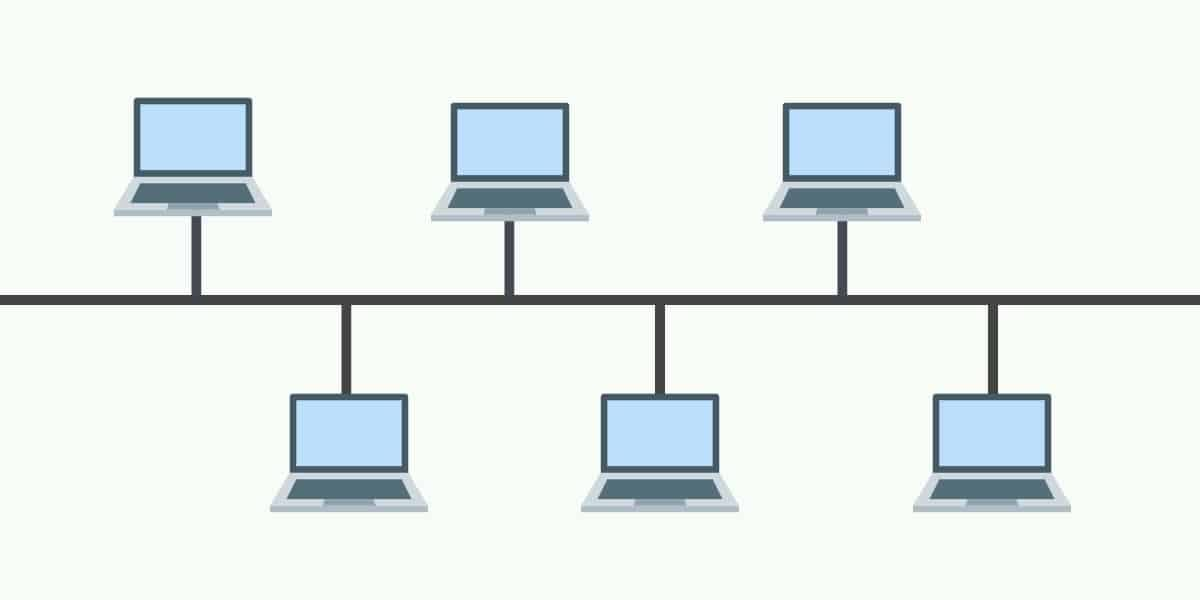
\includegraphics[scale=0.1]{sections/10_kom_roz_dat_sit/images/bus.jpg}
\end{figure}

\paragraph{Kruh}
Každý jeden uzel je připojen ke dvěma dalším. Komunikaci zajišťuje token, který koluje mezi stanicemi 
v jednom směru. Vlastník tokenu může vysílat, ostatní poslouchají (nevznikají kolize). Problém nastane při přerušení kruhu (spoj/stanice).
\begin{figure}[h]
\centering
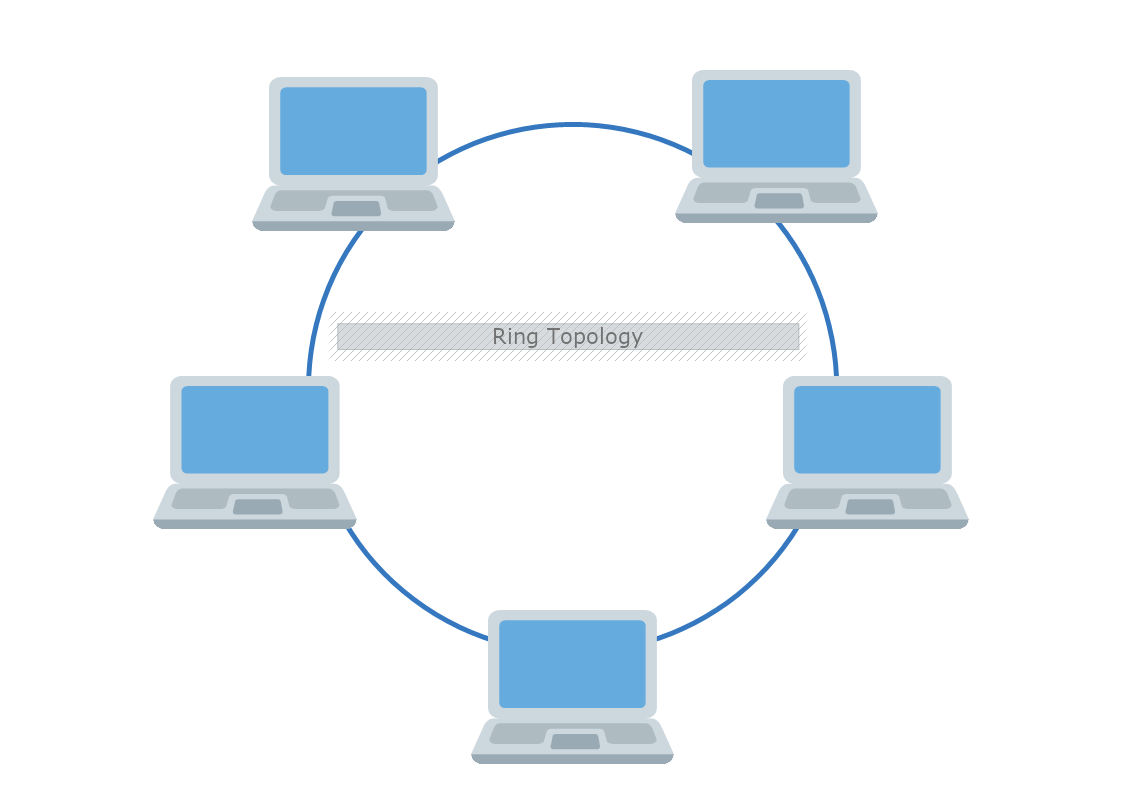
\includegraphics[scale=0.1]{sections/10_kom_roz_dat_sit/images/ring.png}
\end{figure}

\paragraph{Hvězda}
Citlivá na výpadek uzlu. Nejčastější realizace v domácnostech a malých firmách. Odolné proti výpadkům stanic, ale citlivé na výpadek uzlu. Jednoduché rozšíření a řešení závad.
\begin{figure}[h]
\centering
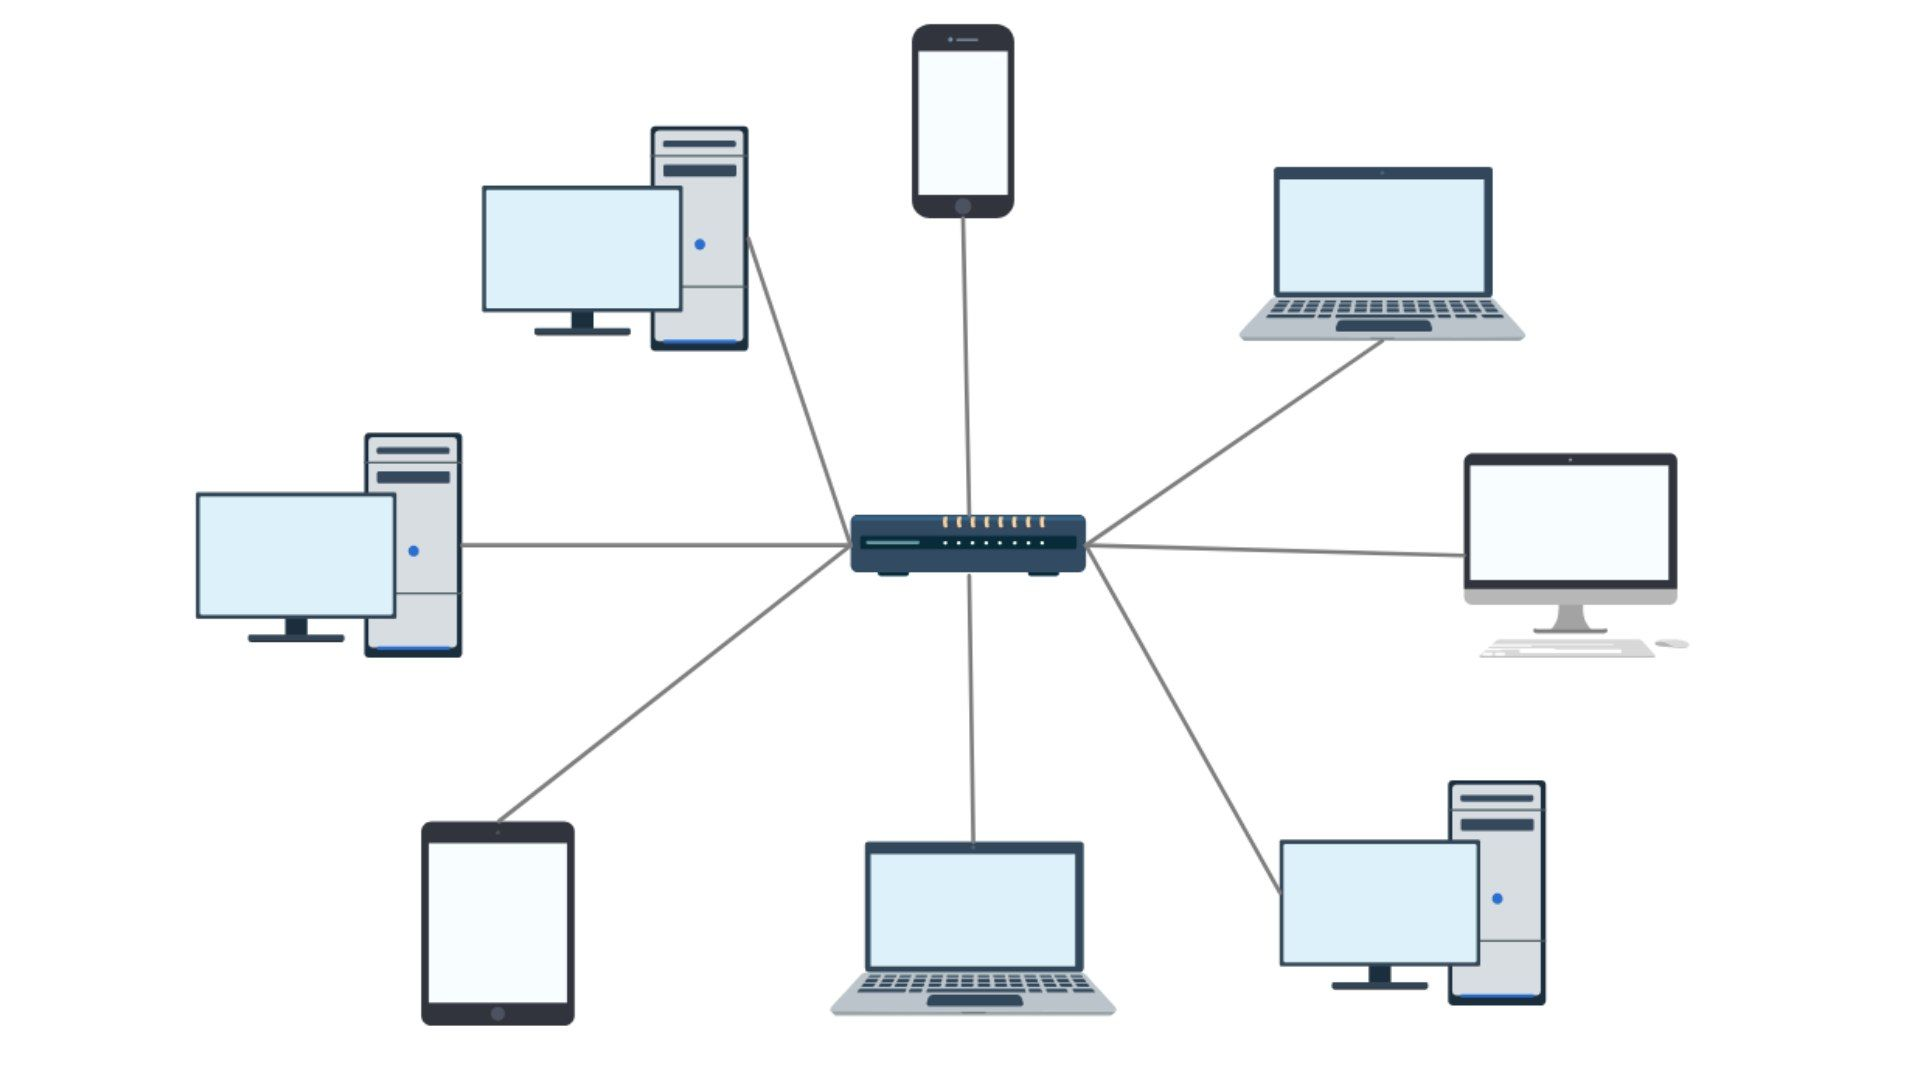
\includegraphics[scale=0.1]{sections/10_kom_roz_dat_sit/images/star.jpg}
\end{figure}

\paragraph{Strom}
Rozšíření hvězdicové topologie propojením aktivních síťových prvků. Používá se ve větších PC sítí. Při selhání jednoho uzlu může sít stále pracovat.
\begin{figure}[h]
\centering
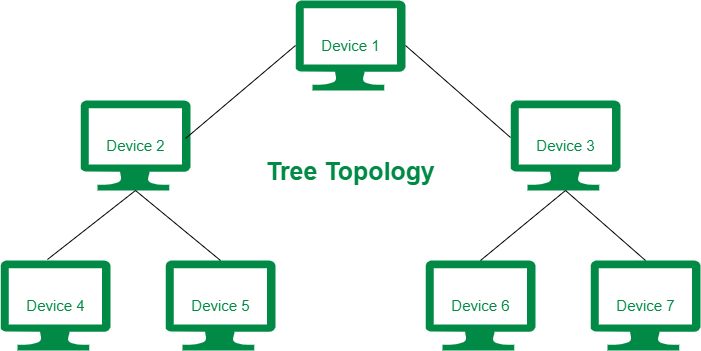
\includegraphics[scale=0.1]{sections/10_kom_roz_dat_sit/images/tree.png}
\end{figure}

\subsection{Popis protokolů}
Carrier Sense Multiple Access with Collision Detection (CSMA/CD) a Carrier Sense Multiple Access with Collision Avoidance (CSMA/CA) jsou dva různé protokoly pro řízení přístupu k médiu (MAC), které se používají v počítačových sítích k řešení problémů s kolizemi při pokusu o přenos dat.
\subsubsection{CSMA/CD}
Carrier Sense Multiple Access with Collision Detection CSMA/CD) je protokol pro přístup k přenosovému médiu v počítačových sítích. Patří do třídy s názvem CSMA. Nejrozšířenějším představitelem CSMA/CD je klasický Ethernet. Ten byl postaven na sběrnicové topologii a algoritmus CSMA/CD v něm řídí přístup stanic ke sdílené sběrnici představované koaxiálním kabelem. Stanice, která chce odeslat datový rámec, se podle jeho pravidel chová následovně: 
\begin{enumerate}
    \item Naslouchá, zda je médium volné. Dokud není, čeká na jeho uvolnění.
    \item Zahájí vysílání. Současně s odesíláním rámce naslouchá, zda nepřichází signál od jiné stanice. Pokud ano, došlo ke kolizi. Stanice ukončí vysílání, odešle signál umožňující rozpoznat kolizi také ostatním (jam signal) a přejde k opakování pokusu podle bodu 3.
    \item Stanice vybere náhodné číslo z intervalu od 0 do 2k - 1, kde k je pořadové číslo pokusu (od 10. pokusu se interval již nezvětšuje a horní hranice zůstává 210 - 1, tedy 1023). Náhodné číslo určuje délku čekací doby, po jejímž uplynutí stanice opakuje pokus o odeslání od bodu 1. Maximální počet pokusů je 16, poté je pokus o odeslání považován za neúspěšný.
\end{enumerate}
Modernější varianty Ethernetu však opouštějí sdílené přenosové médium, používají přepínače s plně duplexním režimem provozu a metoda CSMA/CD u nich není nadále uplatňována. 
\subsubsection{CSMA/CA}
Tento protokol se používá hlavně v bezdrátových sítích, například Wi-Fi. Protokoly skupiny CSMA/CA na rozdíl od CSMA/CD nezjišťují výskyt kolizí (současného vysílání více stanic). Jednotlivé varianty se od sebe mírně odlišují. V CSMA/CA protokolu použitém v síti LocalTalk stanice při volném médiu nejprve ohlásí ostatním, že bude vysílat a médium si tak „zamluví“. Následně odvysílá datový rámec. Bezdrátové sítě standardu 802.11 používají jiný přístup – zde stanice při volném médiu počká náhodně zvolenou dobu a pokud do té doby neobsadí médium někdo jiný, odvysílá datový rámec a následně čeká na jeho potvrzení.
\subsubsection{Token ring}
Token Ring sítě využívají speciální paket, nazývaný token, k informování uzlů o možnosti komunikace. Token je vytvořen při inicializaci sítě. V této fázi jej vytváří buď server, nebo vyčleněná stanice (aktivní monitor, AM). Aktivní monitor sleduje stav tokenu a v případě jeho ztráty nebo poškození vygeneruje nový.

Pohotovostní monitor (SM) hlídá aktivní monitor a v případě nutnosti jej zastoupí, čímž se stává novým aktivním monitorem. Token má velikost 3 bajty.

\paragraph{Princip komunikace} 
Vysílat může pouze ten uzel, který má právě prázdný (idle) token. Stanice označí token jako zaneprázdněný (busy) a spolu s daty jej předá sousední stanici. Tento proces pokračuje, dokud token a data nedorazí k cílové stanici. Příjemce potvrzuje přijetí dat zasláním označeného tokenu zpět odesílateli. Po potvrzení odesílatel obnoví token do původního prázdného stavu, což umožňuje další vysílání.

\paragraph{Nahrazení Ethernetem} 
Token Ring technologie byla postupně nahrazena Ethernetem. Ethernet nabízí jednodušší architekturu, vyšší rychlosti a nižší náklady na implementaci a údržbu. Ethernet také lépe podporuje různé topologie a je dnes dominantní technologií pro LAN sítě.

\subsection{Kabeláž}
\paragraph{10Base5}
10Base5 (nebo též Tlustý Ethernet nebo Žlutý kabel) je označení historicky nejstarší verze Ethernetu. Pracuje s rychlostí 10 Mbit/s, dovoluje vytvářet segmenty délky až 500 metrů s nejvýše 100 počítači. Označení „Tlustý“ (anglicky „Thick“) si vysloužil díky poměrně velké tloušťce použitého kabelu stejně jako označení „žlutý“ (kabel měl žlutou barvu). 10Base5 je realizováno pomocí koaxiálního kabelu o impedanci 50 ohm a průměru 0,4 palce (přibližně 10 mm). Nástupcem byla technologie 10Base2 („tenký Ethernet“). 

\paragraph{10Base2}
10Base2 (také 10BASE2, často nazýván též tenký Ethernet) je standard sítě Ethernet založený na tenkém koaxiálním kabelu s rychlostí přenosu 10 Mbit/s a vzdáleností mezi uzly maximálně 185 metrů. Používá sběrnicovou topologii a tenký 50 ohm koaxiální kabel (RG-58). Na jednom segmentu může být maximálně 30 počítačů, vzdálenost mezi odbočkami je minimálně 50 centimetrů, délka kabelu od odbočky k síťové kartě je maximálně 30 centimetrů. 

\paragraph{10BaseT}
10BASE-T je označení překonaného standardu sítě Ethernet, který používá dva páry kroucené dvojlinky Cat-3 nebo Cat-5.

\paragraph{Přímý vs. křížený kabel}
Jestliže jsou zařízení spojena přímo, je nutné použít křížený kabel. Pokud jsou zařízení připojena přes aktivní prvek (hub nebo switch), každé z nich je do tohoto aktivního prvku připojeno přímým kabelem.
\subsection{ISO/OSI model}
ISO/OSI model poskytuje standardizovaný přístup k návrhu a porozumění síťových architektur, čímž usnadňuje interoperabilitu a komunikaci mezi různými síťovými zařízeními a systémy. Je konceptuální rámec, který standardizuje funkce sítě do sedmi vrstev, aby umožnil interoperabilitu různých systémů a technologií. Jednotlivé vrstvy modelu jsou:

\paragraph{1. Fyzická vrstva (Physical Layer)} Tato vrstva se zabývá fyzickým přenosem bitů přes různé druhy médií, jako jsou kabely a rádiové vlny. Zahrnuje specifikace pro konektory, napětí, kabeláže a topologie.

\paragraph{2. Spojová vrstva (Data Link Layer)} Tato vrstva zajišťuje spolehlivý přenos datových rámců mezi dvěma uzly v rámci stejné sítě. Řeší chyby, řízení toku dat a MAC adresování.

\paragraph{3. Síťová vrstva (Network Layer)} Síťová vrstva je zodpovědná za směrování paketů mezi uzly v různých sítích. Používá IP adresy a směrovací protokoly k nalezení optimální cesty pro přenos dat.

\paragraph{4. Transportní vrstva (Transport Layer)} Tato vrstva poskytuje spolehlivý přenos dat mezi koncovými zařízeními. Používá protokoly jako TCP a UDP k řízení spojení, segmentaci a znovuskládání datových segmentů.

\paragraph{5. Relační vrstva (Session Layer)} Relační vrstva řídí a udržuje spojení mezi aplikacemi na různých zařízeních. Zajišťuje synchronizaci a řízení dialogu mezi komunikujícími aplikacemi.

\paragraph{6. Prezentační vrstva (Presentation Layer)} Tato vrstva zajišťuje formátování a kódování dat tak, aby byla srozumitelná pro aplikace. Provádí kompresi dat, šifrování a překlad mezi různými formáty dat.

\paragraph{7. Aplikační vrstva (Application Layer)} Aplikační vrstva je nejbližší uživateli a zajišťuje služby, které přímo podporují různé síťové aplikace. Zahrnuje protokoly jako HTTP, FTP, SMTP a další, které umožňují komunikaci mezi aplikacemi.

\subsection{TCP/IP Model}
TCP/IP model je méně striktní a skládá se z čtyř vrstev, které popisují operace potřebné pro síťovou komunikaci.

\paragraph{1. Síťová vrstva (Internet Layer}
Obdobná síťové vrstvě ISO/OSI modelu, zajišťuje směrování a adresaci.
\paragraph{2. Transportní vrstva (Transport Layer)}
Zahrnuje funkce transportní vrstvy ISO/OSI modelu, ale je méně specifická.
\paragraph{3. Aplikační vrstva (Application Layer)}
Shoduje se s aplikační vrstvou ISO/OSI modelu, ale je méně podrobná.
\paragraph{4. Rozhraní sítě (Network Interface Layer)}
Tato vrstva v TCP/IP modelu kombinuje aspekty fyzické a spojové vrstvy ISO/OSI modelu.

\paragraph{Srovnání ISO OSI modelu s TCP/IP modelem}
ISO/OSI model poskytuje podrobnější rozdělení síťových funkcí, zatímco TCP/IP model je jednodušší a méně specifikovaný. TCP/IP model vznikl jako praktický nástroj pro implementaci Internetu, zatímco ISO/OSI model byl navržen jako univerzální rámec pro síťovou komunikaci. TCP/IP model je dominantní v praxi pro implementaci a konfiguraci sítí, zatímco ISO/OSI model spíše slouží jako referenční rámec pro teoretické studium síťových protokolů. Dnes je TCP/IP model dominantním rámcem pro návrh, implementaci a správu moderních sítí a internetu. ISO/OSI model stále slouží jako teoretický referenční rámec, ale jeho praktické využití v praxi je omezené, především v oblasti konkrétních implementací a konfigurací sítí.